\documentclass[a4paper,12pt,oneside]{book}
%
\let\proof\relax
\let\endproof\relax
\usepackage{amsthm}
\usepackage{graphicx,rotating}
\usepackage{complexity}
\usepackage{tikz}
\usepackage{xspace}
\usepackage{fix-cm}
\usetikzlibrary{shadows}
\usetikzlibrary{shapes,positioning,arrows}
\usetikzlibrary{decorations.pathmorphing}
\usetikzlibrary{shadows,arrows,patterns,automata,calc,intersections,fit,shapes.misc, decorations.markings}
\usepackage[underline=false,rounded corners=true]{pgf-umlsd}
\usepackage{todonotes}
\usepackage{paralist}
%\usepackage{parskip} % Creates paragraphs - Maybe remove for more space
\setdefaultenum{1)}{(a)}{i)}{A)}
\usepackage{multicol}% http://ctan.org/pkg/multicols
\usepackage{multirow}

\usepackage{lmodern}
\usepackage[brazilian]{babel}

% \usepackage{msc}
% \usepackage[
% n,
% operators,
% advantage,
% sets,
% adversary,
% landau,
% probability,
% notions,
% logic,
% ff,
% mm,
% primitives,
% events,
% complexity,
% asymptotics,
% keys]{cryptocode}
% \usepackage{dashbox}

\usepackage[
%pdfauthor={},
%pdfsubject={},
%pdftitle={},
%pdfkeywords={},
bookmarks=false,
breaklinks=true,
colorlinks=true,
linkcolor=black,
citecolor=black,
urlcolor=black,
%pdfstartpage=19,
pdfpagelayout=SinglePage
]{hyperref}
%enables correct jumping to figures when referencing
\usepackage[all]{hypcap}

\usepackage{dsfont}
\usepackage[bottom]{footmisc}
\usepackage[nocompress]{cite}
\usepackage{listings}
\usepackage{fancyvrb}
\usepackage{bm}
\usepackage{amssymb}
\usepackage{amsmath}
\usepackage{cleveref}
\usepackage{mathtools}
% \usepackage{algorithm}
% \usepackage{algorithmic}
\usepackage{etoolbox}
\usepackage{varwidth} %for the varwidth minipage environment
\usepackage{array} % for defining a new column type
\usepackage{chngcntr}
\usepackage{stmaryrd}
\usepackage{tabulary}
\usepackage{booktabs}

\usepackage{wrapfig,epsfig}

\usepackage{xcolor}% http://ctan.org/pkg/xcolor
\usepackage{graphicx}
\usepackage{color}
\usepackage{todonotes}
% Fonts
\usepackage{microtype}
\usepackage[T1]{fontenc}
\usepackage{textcomp}
\usepackage[utf8]{inputenc}
\usepackage{inconsolata}

\usepackage{enumitem}

%B-Method packages
% \usepackage{eventB}
% \usepackage{zed-csp}

% \usepackage[linesnumbered, ruled, noend]{algorithm2e} % algorithms
% \usepackage{algorithmicx}

\usepackage{float}
\usepackage{listing}
\usepackage{mdframed}
% \usepackage{subcaption}
\usepackage{caption}
% \usepackage{draftwatermark}
% \SetWatermarkScale{1}

% Referencing
\newcommand{\Fref}[1]{Figure~\ref{#1}}
\newcommand{\fref}[1]{figure~\ref{#1}}

\newcommand{\Tref}[1]{Table~\ref{#1}}
\newcommand{\tref}[1]{table~\ref{#1}}

\newcommand{\Eref}[1]{Equation~\ref{#1}}
\newcommand{\eref}[1]{equation~\ref{#1}}

\newcommand{\Sref}[1]{Section~\ref{#1}}
\newcommand{\sref}[1]{section~\ref{#1}}

\newcommand{\Lref}[1]{Listing~\ref{#1}}
\newcommand{\lref}[1]{listing~\ref{#1}}

% names
\newcommand{\otoken}{O\textsc{-token}\xspace}
\newcommand{\otokens}{O\textsc{-tokens}\xspace}
\newcommand{\otokenFull}{O\textsc{bscure} T\textsc{oken}\xspace}

% Messages
\newcommand{\osrreq}{O\textsc{sr-req}\xspace}
\newcommand{\osrconf}{O\textsc{sr-conf}\xspace}


% SRS cover page
\title{
  \begin{flushright}
  \Huge{MODELO FÍSICO ESTRUTURAL,}\\
  ASSERTIVAS\\
  e\\
  EXEMPLO FÍSICO\\
  da aplicação\\
  LABIRINTO\\
  ~\\
  \LARGE{Versão 2.0}\\
  ~\\
  INF1301 - Programação Modular\\ DI/PUC-Rio
  \end{flushright}
}

% Author
\author{Antônio Chaves - AVC\\João Pedro Paiva - JPP\\Pedro Costa - PC}
\date{\today}

\begin{document}

\frontmatter
\maketitle

\tableofcontents

\chapter*{Histórico de Revisões}

\begin{center}
    \begin{tabular}{|c|c|c|c|}
        \hline
        Versão & Data       & Autor & Observações                                      \\
        \hline
        1.0    & 08/10/2019 & AVC   & Versão do Trab2                                  \\
        \hline
    \end{tabular}
\end{center}


\mainmatter

\chapter{Modelo Físico Estrutural}

\begin{center}

    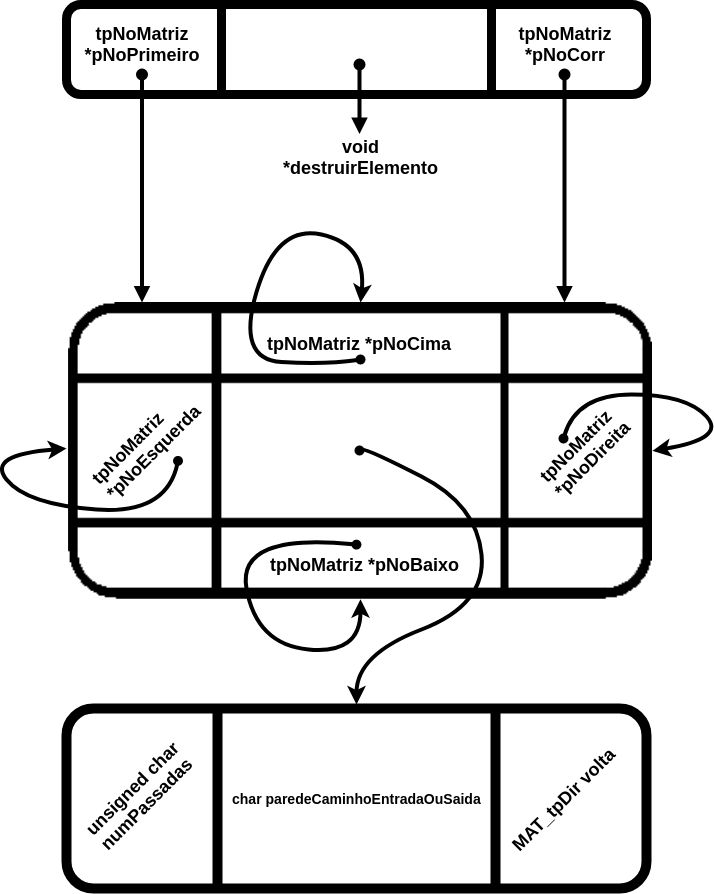
\includegraphics[width=1\textwidth,height=27\baselineskip]{fisico.png}

\end{center}

\chapter{Assertivas Estruturais}\setlength{\parskip}{1\baselineskip}

    Se o pNoCorr->pNoDireita diferente de NULL, então pNoCorr->pNoDireita->pNoEsquerda = pNoCorr;

    Se o pNoCorr->pNoEsquerda diferente de NULL, então pNoCorr->pNoEsquerda->pNoDireita = pNoCorr;

    Se o pNoCorr->pNoCima diferente de NULL, então pNoCorr->pNoCima->pNoBaixo = pNoCorr;

    Se o pNoCorr->pNoBaixo diferente de NULL, então pNoCorr->pNoBaixo->pNoCima = pNoCorr;
    \setlength{\parskip}{1pt}
\chapter{Exemplo Físico}

\begin{center}
    
    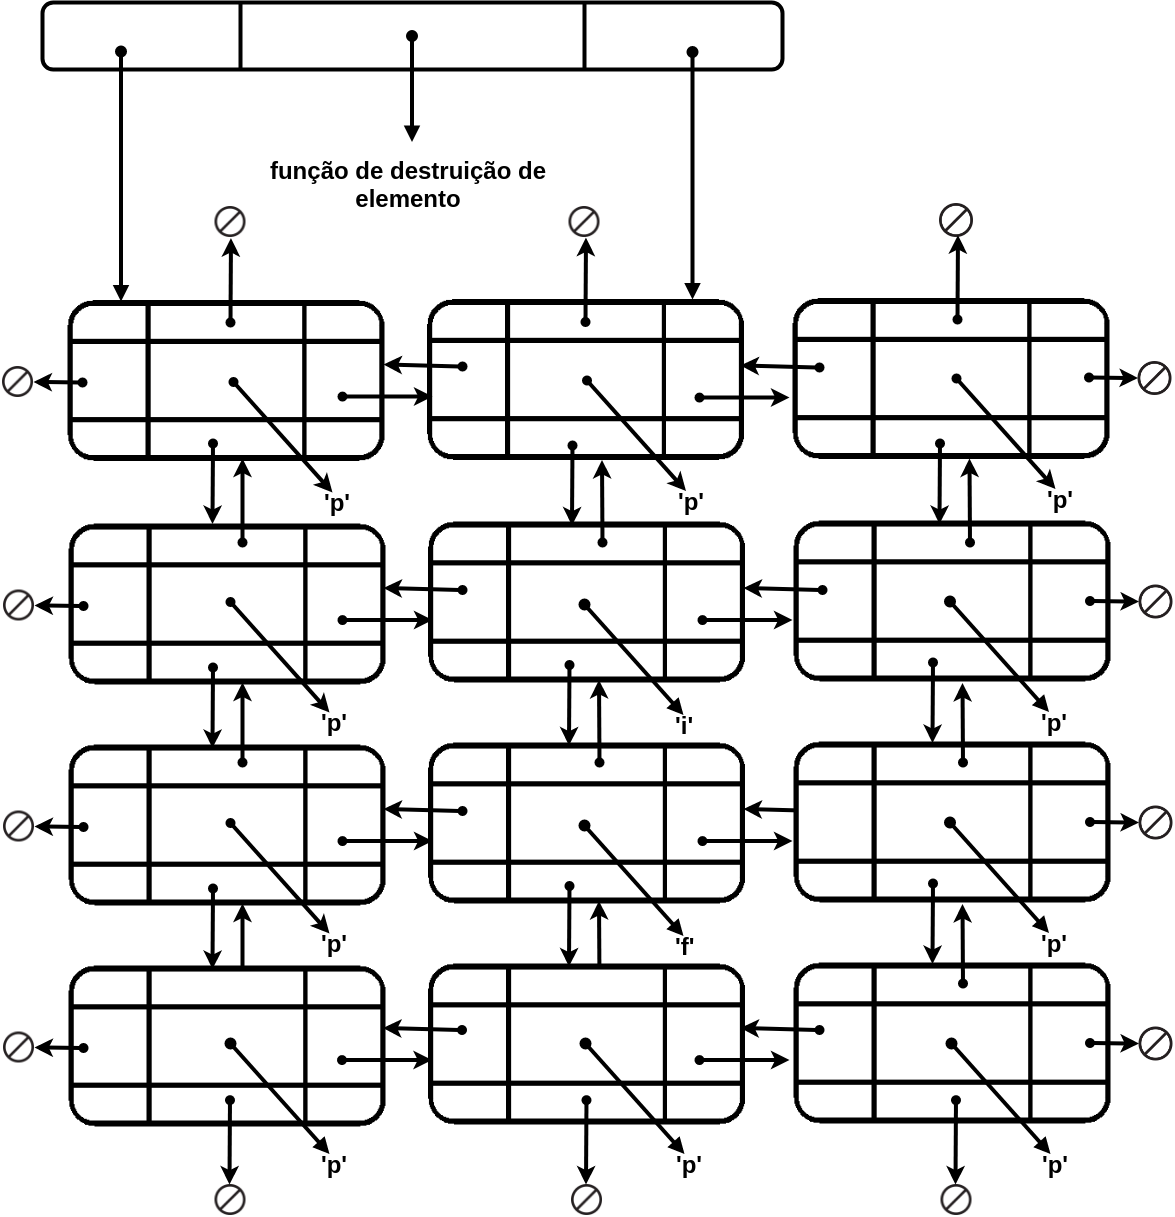
\includegraphics[width=\textwidth,height=27\baselineskip]{exemplo.png}

\end{center}

% \chapter*{Preface}
Lorem ipsum dolor sit amet.


\section*{Structure of Specification}
% You might want to add short description about each chapter in this book.
Each unit will focus on <SOMETHING>.

% \chapter{Introdução}

\section{Objetivo}
$<$Identify the product whose software requirements are specified in this
document, including the revision or release number. Describe the scope of the
product that is covered by this SRS, particularly if this SRS describes only
part of the system or a single subsystem.$>$

\section{Document Conventions}
$<$Describe any standards or typographical conventions that were followed when
writing this SRS, such as fonts or highlighting that have special significance.
For example, state whether priorities  for higher-level requirements are assumed
to be inherited by detailed requirements, or whether every requirement statement
is to have its own priority.$>$

\section{Intended Audience and Reading Suggestions}
$<$Describe the different types of reader that the document is intended for,
such as developers, project managers, marketing staff, users, testers, and
documentation writers. Describe what the rest of this SRS contains and how it is
organized. Suggest a sequence for reading the document, beginning with the
overview sections and proceeding through the sections that are most pertinent to
each reader type.$>$

\section{Project Scope}
$<$Provide a short description of the software being specified and its purpose,
including relevant benefits, objectives, and goals. Relate the software to
corporate goals or business strategies. If a separate vision and scope document
is available, refer to it rather than duplicating its contents here.$>$

\section{References}
$<$List any other documents or Web addresses to which this SRS refers. These may
include user interface style guides, contracts, standards, system requirements
specifications, use case documents, or a vision and scope document. Provide
enough information so that the reader could access a copy of each reference,
including title, author, version number, date, and source or location.$>$

% \chapter{Descrição Geral}

\section{Perspectiva do Produto}
% $<$Describe the context and origin of the product being specified in this SRS.
% For example, state whether this product is a follow-on member of a product
% family, a replacement for certain existing systems, or a new, self-contained
% product. If the SRS defines a component of a larger system, relate the
% requirements of the larger system to the functionality of this software and
% identify interfaces between the two. A simple diagram that shows the major
% components of the overall system, subsystem interconnections, and external
% interfaces can be helpful.$>$
A aplicação Labirinto é completamente autocontida, não é um componente de outro sistema.

\section{Funções do Projeto}
% $<$Summarize the major functions the product must perform or must let the user
% perform. Details will be provided in Section 3, so only a high level summary
% (such as a bullet list) is needed here. Organize the functions to make them
% understandable to any reader of the SRS. A picture of the major groups of
% related requirements and how they relate, such as a top level data flow diagram
% or object class diagram, is often effective.$>$
Será possível construir manualmente um labirinto através de funções específicas (com apenas quatro direções a serem tomadas a cada decisão: norte, sul, leste, oeste) e uma função adicional deverá imprimir o caminho da entrada até a saída.

% \section{User Classes and Characteristics}
% $<$Identify the various user classes that you anticipate will use this product.
% User classes may be differentiated based on frequency of use, subset of product
% functions used, technical expertise, security or privilege levels, educational
% level, or experience. Describe the pertinent characteristics of each user class.
% Certain requirements may pertain only to certain user classes. Distinguish the
% most important user classes for this product from those who are less important
% to satisfy.$>$

\section{Ambiente de Operação}
% $<$Describe the environment in which the software will operate, including the
% hardware platform, operating system and versions, and any other software
% components or applications with which it must peacefully coexist.$>$
A aplicação deve operar em computadores 64-bit com OS Windows 7, 8 e 10.

\section{Restrições de Design e Implementação}
% $<$Describe any items or issues that will limit the options available to the
% developers. These might include: corporate or regulatory policies; hardware
% limitations (timing requirements, memory requirements); interfaces to other
% applications; specific technologies, tools, and databases to be used; parallel
% operations; language requirements; communications protocols; security
% considerations; design conventions or programming standards (for example, if the
% customer’s organization will be responsible for maintaining the delivered
% software).$>$
A aplicação Labirinto deve ser desenvolvida por completo utilizando a linguagem de programação C. Será obrigatório que a arquitetura da aplicação tenha pelo menos dois tipos abstratos de dados (um pode utilizar o outro) além de um módulo centralizador principal. É proibida a utilização de LISTAS
ENCADEADAS e QUALQUER ESTRUTURA ESTÁTICA (por exemplo: VETORES ESTÁTICOS). O algorítmo de resolução do labirinto é... Todos os programas devem estar em conformidade com os padrões dos apêndices de 1 a 10 do livro-texto da disciplina. Em particular, os módulos e funções devem estar devidamente especificados.

\section{User Documentation}
$<$List the user documentation components (such as user manuals, on-line help,
and tutorials) that will be delivered along with the software. Identify any
known user documentation delivery formats or standards.$>$

\section{Suposições e Dependências}
% $<$List any assumed factors (as opposed to known facts) that could affect the
% requirements stated in the SRS. These could include third-party or commercial
% components that you plan to use, issues around the development or operating
% environment, or constraints. The project could be affected if these assumptions
% are incorrect, are not shared, or change. Also identify any dependencies the
% project has on external factors, such as software components that you intend to
% reuse from another project, unless they are already documented elsewhere (for
% example, in the vision and scope document or the project plan).$>$
A versão final da aplicação Labirinto, a ser completada no Trabalho 3, rodará fora do arcabouço
com uma interface com o usuário, ou seja, terá um módulo principal.

% \chapter{Requerimentos de Interface Externa}

\section{Interface de Usuârio}
% $<$Describe the logical characteristics of each interface between the software
% product and the users. This may include sample screen images, any GUI standards
% or product family style guides that are to be followed, screen layout
% constraints, standard buttons and functions (e.g., help) that will appear on
% every screen, keyboard shortcuts, error message display standards, and so on.
% Define the software components for which a user interface is needed. Details of
% the user interface design should be documented in a separate user interface
% specification.$>$

O usuário deve ser capaz de construir o labirinto manulamente, escrevendo em um arquivo txt que será salvo e lido pelo programa. O labirinto e sua solução devem ser gerados pela aplicação e mostrados para o usuário graficamente utilizando caracteres ascii para compor a figura.

% \section{Hardware Interfaces}
% $<$Describe the logical and physical characteristics of each interface between
% the software product and the hardware components of the system. This may include
% the supported device types, the nature of the data and control interactions
% between the software and the hardware, and communication protocols to be
% used.$>$

% \section{Software Interfaces}
% $<$Describe the connections between this product and other specific software
% components (name and version), including databases, operating systems, tools,
% libraries, and integrated commercial components. Identify the data items or
% messages coming into the system and going out and describe the purpose of each.
% Describe the services needed and the nature of communications. Refer to
% documents that describe detailed application programming interface protocols.
% Identify data that will be shared across software components. If the data
% sharing mechanism must be implemented in a specific way (for example, use of a
% global data area in a multitasking operating system), specify this as an
% implementation constraint.$>$

% \section{Communications Interfaces}
% $<$Describe the requirements associated with any communications functions
% required by this product, including e-mail, web browser, network server
% communications protocols, electronic forms, and so on. Define any pertinent
% message formatting. Identify any communication standards that will be used, such
% as FTP or HTTP. Specify any communication security or encryption issues, data
% transfer rates, and synchronization mechanisms.$>$

% \chapter{Funcionalidades do Sistema}
% $<$This template illustrates organizing the functional requirements for the
% product by system features, the major services provided by the product. You may
% prefer to organize this section by use case, mode of operation, user class,
% object class, functional hierarchy, or combinations of these, whatever makes the
% most logical sense for your product.$>$

\section{Funcionalidade 1}
% $<$Don’t really say “System Feature 1.” State the feature name in just a few
% words.$>$

Constrói labirinto.

\subsection{Descrição e Prioridade}
% $<$Provide a short description of the feature and indicate whether it is of
% High, Medium, or Low priority. You could also include specific priority
% component ratings, such as benefit, penalty, cost, and risk (each rated on a
% relative scale from a low of 1 to a high of 9).$>$

Funcionalidade que constrói o labirinto a ser resolvido. Prioridade alta. Funcionalidade essencial para o funcionamento da aplicação.

\subsection{Stimulus/Response Sequences}
% $<$List the sequences of user actions and system responses that stimulate the
% behavior defined for this feature. These will correspond to the dialog elements
% associated with use cases.$>$
O usuário contrói o labirinto manulamente, escrevendo em um arquivo txt. Ao rodar a aplicação Labirinto, o labirinto salvo no txt é armazenado numa matriz criada pelo módulo Matriz.

\subsection{Functional Requirements}
$<$Itemize the detailed functional requirements associated with this feature.
These are the software capabilities that must be present in order for the user
to carry out the services provided by the feature, or to execute the use case.
Include how the product should respond to anticipated error conditions or
invalid inputs. Requirements should be concise, complete, unambiguous,
verifiable, and necessary. Use “TBD” as a placeholder to indicate when necessary
information is not yet available.$>$

$<$Each requirement should be uniquely identified with a sequence number or a
meaningful tag of some kind.$>$

REQ-1:	REQ-2:

\section{Funcionalidade 2}
% $<$Don’t really say “System Feature 1.” State the feature name in just a few
% words.$>$

Resolve labirinto.

\subsection{Descrição e Prioridade}
% $<$Provide a short description of the feature and indicate whether it is of
% High, Medium, or Low priority. You could also include specific priority
% component ratings, such as benefit, penalty, cost, and risk (each rated on a
% relative scale from a low of 1 to a high of 9).$>$

Funcionalidade que resolve o labirinto construído. Prioridade alta. Funcionalidade essencial para o funcionamento da aplicação.

\subsection{Stimulus/Response Sequences}
$<$List the sequences of user actions and system responses that stimulate the
behavior defined for this feature. These will correspond to the dialog elements
associated with use cases.$>$

\subsection{Functional Requirements}
$<$Itemize the detailed functional requirements associated with this feature.
These are the software capabilities that must be present in order for the user
to carry out the services provided by the feature, or to execute the use case.
Include how the product should respond to anticipated error conditions or
invalid inputs. Requirements should be concise, complete, unambiguous,
verifiable, and necessary. Use “TBD” as a placeholder to indicate when necessary
information is not yet available.$>$

$<$Each requirement should be uniquely identified with a sequence number or a
meaningful tag of some kind.$>$

REQ-1:	REQ-2:

\section{Funcionalidade 3}
% $<$Don’t really say “System Feature 1.” State the feature name in just a few
% words.$>$

Imprime solução labirinto.

\subsection{Descrição e Prioridade}
% $<$Provide a short description of the feature and indicate whether it is of
% High, Medium, or Low priority. You could also include specific priority
% component ratings, such as benefit, penalty, cost, and risk (each rated on a
% relative scale from a low of 1 to a high of 9).$>$

Funcionalidade que imprime o labirinto resolvido com o caminho do início até o fim demarcado. Prioridade alta. Funcionalidade essencial para o funcionamento da aplicação.

\subsection{Stimulus/Response Sequences}
$<$List the sequences of user actions and system responses that stimulate the
behavior defined for this feature. These will correspond to the dialog elements
associated with use cases.$>$

\subsection{Functional Requirements}
$<$Itemize the detailed functional requirements associated with this feature.
These are the software capabilities that must be present in order for the user
to carry out the services provided by the feature, or to execute the use case.
Include how the product should respond to anticipated error conditions or
invalid inputs. Requirements should be concise, complete, unambiguous,
verifiable, and necessary. Use “TBD” as a placeholder to indicate when necessary
information is not yet available.$>$

$<$Each requirement should be uniquely identified with a sequence number or a
meaningful tag of some kind.$>$

REQ-1:	REQ-2:
% \chapter{Outros Requisitos}

\section{Hipóteses}
O labirinto criado pelo usuário tem dimensões de no máximo 10x10.

O labirinto criado pelo usuário possui início e fim.

A posição do início do labirinto não é a mesma que a do fim do labirinto.

% \section{Performance Requirements}
% $<$If there are performance requirements for the product under various
% circumstances, state them here and explain their rationale, to help the
% developers understand the intent and make suitable design choices. Specify the
% timing relationships for real time systems. Make such requirements as specific
% as possible. You may need to state performance requirements for individual
% functional requirements or features.$>$

% \section{Safety Requirements}
% $<$Specify those requirements that are concerned with possible loss, damage, or
% harm that could result from the use of the product. Define any safeguards or
% actions that must be taken, as well as actions that must be prevented. Refer to
% any external policies or regulations that state safety issues that affect the
% product’s design or use. Define any safety certifications that must be
% satisfied.$>$

% \section{Security Requirements}
% $<$Specify any requirements regarding security or privacy issues surrounding use
% of the product or protection of the data used or created by the product. Define
% any user identity authentication requirements. Refer to any external policies or
% regulations containing security issues that affect the product. Define any
% security or privacy certifications that must be satisfied.$>$

% \section{Software Quality Attributes}
% $<$Specify any additional quality characteristics for the product that will be
% important to either the customers or the developers. Some to consider are:
% adaptability, availability, correctness, flexibility, interoperability,
% maintainability, portability, reliability, reusability, robustness, testability,
% and usability. Write these to be specific, quantitative, and verifiable when
% possible. At the least, clarify the relative preferences for various attributes,
% such as ease of use over ease of learning.$>$

% \section{Business Rules}
% $<$List any operating principles about the product, such as which individuals or
% roles can perform which functions under specific circumstances. These are not
% functional requirements in themselves, but they may imply certain functional
% requirements to enforce the rules.$>$

% \chapter{Other Requirements}
$<$Define any other requirements not covered elsewhere in the SRS. This might
include database requirements, internationalization requirements, legal
requirements, reuse objectives for the project, and so on. Add any new sections
that are pertinent to the project.$>$

\section{Appendix A: Glossary}
%see https://en.wikibooks.org/wiki/LaTeX/Glossary
$<$Define all the terms necessary to properly interpret the SRS, including
acronyms and abbreviations. You may wish to build a separate glossary that spans
multiple projects or the entire organization, and just include terms specific to
a single project in each SRS.$>$

\section{Appendix B: Analysis Models}
$<$Optionally, include any pertinent analysis models, such as data flow
diagrams, class diagrams, state-transition diagrams, or entity-relationship
diagrams.$>$

\section{Appendix C: To Be Determined List}
$<$Collect a numbered list of the TBD (to be determined) references that remain
in the SRS so they can be tracked to closure.$>$


\end{document}
